
\title{15-440: Lab 2}
\author{
        Spencer Barton (sebarton)\\
        Emma Binns (ebinns)
}
\date{September 11, 2014}

\documentclass[12pt]{article}

\usepackage{graphicx}
\usepackage[compact]{titlesec}

\setlength{\parindent}{0pt}
\setlength{\parskip}{\baselineskip}

\begin{document}
\maketitle

%------------------------------------------

\section{Design}

- UML diagram (Emma)
- Why no skeleton

\subsection*{Registry Lookup}

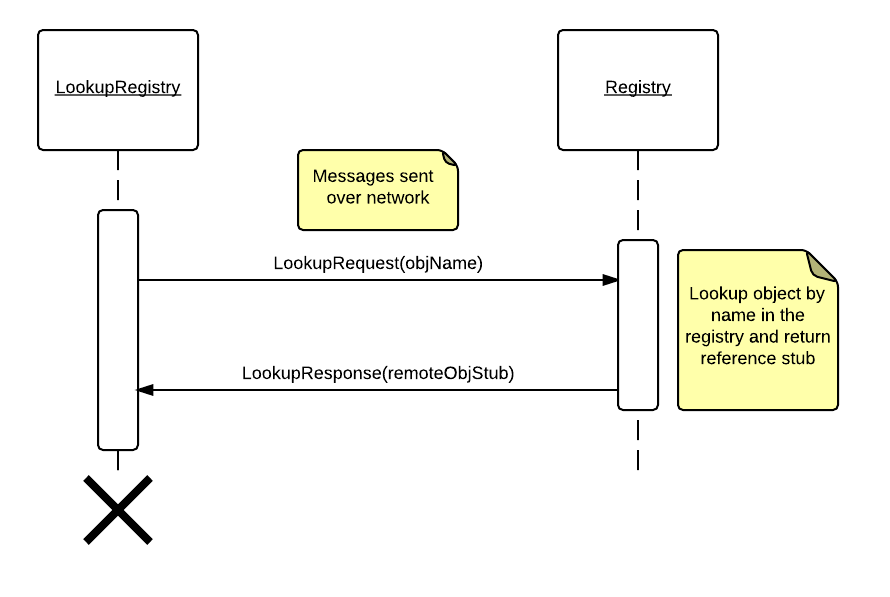
\includegraphics[scale=.4]{Lookup.png}

In order to lookup a remote object the client uses their \texttt{LookupRegistry} to lookup an object by name string. The \texttt{LookupRegistry} creates a \texttt{LookupRequest} with the object name. This is sent to the server which looks up the object by name in its registry. If the object exists, a \texttt{RemoteObjectStub} is returned through a \texttt{LookupResponse} else the \texttt{LookupResponse} comes back with an exception.

\subsection*{Remote Method Invocation}

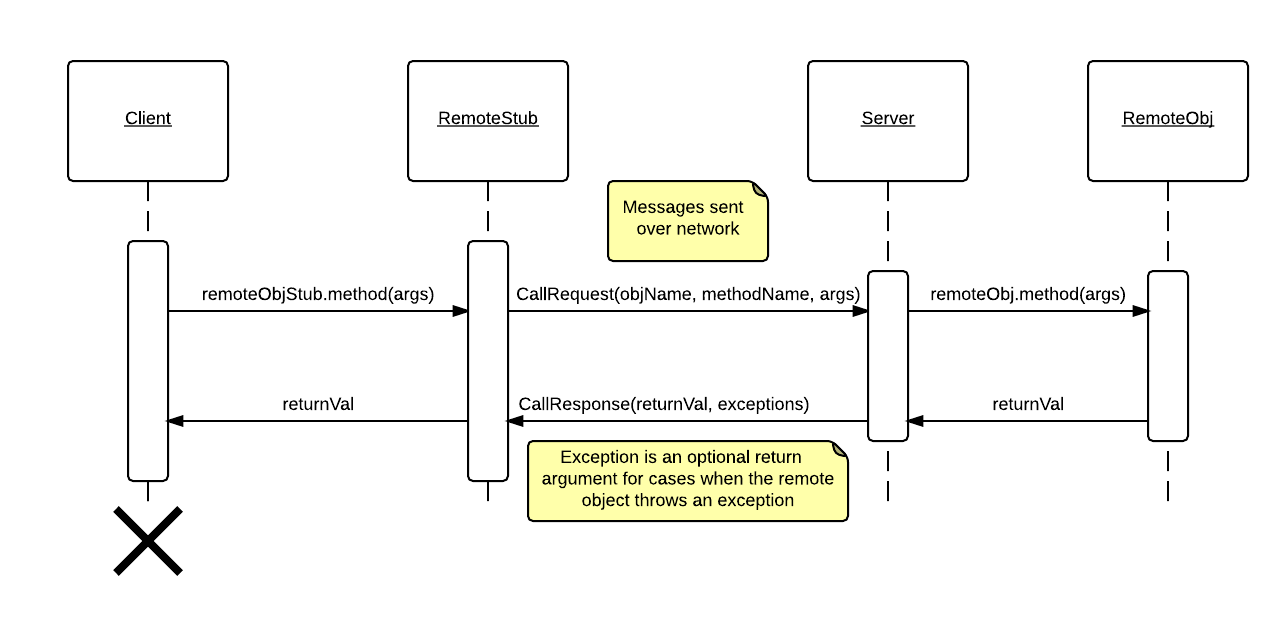
\includegraphics[scale=.3]{callMethod.png}


%------------------------------------------

\section{Implementation State}

We completed the basic requirements.

The extras that were not added include a skeleton, compiler and loading class files. We chose not to implement skeletons as we were able to add that the necessary methods within \texttt{RemoteObject}.

In order to add a compiler the design would not need to change. When performing a registry lookup a remote object stub is returned. Currently this remote object stub must be instantiated earlier by the server. With a compiler this would simply be replaced by a call to the compiler during an object lookup.

Finally support for loading class files would require a little more work since another server socket would need to be implemented on the host the .class files. Beyond that the remote object stub would handle a .class request and another type of message could be implemented to handle this communication.

%------------------------------------------

\section{Running the Project}

- Instructions (example run)
- CHECK works Andrew machines
(Emma)

%------------------------------------------

\section{Dependencies}

There are no dependencies.

%------------------------------------------

\section{Testing}

Our test in built into \texttt{PartyClient}. It automatically runs when \texttt{PartyClient} is run. The test runs each of the methods in the \texttt{Person} object for both a remote and local implementation. \texttt{Person.samePerson} is run using both remote and local objects as arguments to check that the server-side remote object implementation can handle either object type as an argument.

\end{document}
